% Results section

% \subsection{Primary findings}

% [Primary results and findings]

% % Demo table: descriptive statistics for the synthetic outcome measure.
% % The component file wraps the raw tabular in assets/tables/ with a caption and label.
% Table~\ref{tab:demo-descriptive} reports demo descriptive statistics across the four study conditions.
% % source: assets/tables/tab_demo_descriptive.tex
\begin{table}[H]
  \centering
  \caption{
    % table scope
    \textbf{Demo descriptive statistics across study conditions.}
    % table contents
    Per-condition summary of the synthetic outcome measure, reporting
    sample size, mean, standard deviation, and 95\% confidence interval
    for the mean. Values are illustrative only and exist to demonstrate
    the assets/components layout used by this template.
  }
  \label{tab:demo-descriptive}
  \small
  \begin{tabular}{lrrrr}
\toprule
Condition & N & Mean & SD & 95\% CI \\
\midrule
Control       & 30 & 12.4 & 2.8 & (11.4, 13.4) \\
Treatment A   & 32 & 15.7 & 3.1 & (14.6, 16.8) \\
Treatment B   & 31 & 14.9 & 2.9 & (13.9, 15.9) \\
Treatment A+B & 29 & 18.2 & 3.4 & (16.9, 19.5) \\
\bottomrule
\end{tabular}

\end{table}


% % Demo figure: matching visual summary.
% % The component file wraps the figure asset in assets/figures/ with a caption and label.
% Figure~\ref{fig:demo-colorbox} visualises the same per-condition means.
% % source: assets/figures/fig_demo_colorbox.pdf
\begin{figure}[H]
  \centering
  \begin{minipage}{\textwidth}
  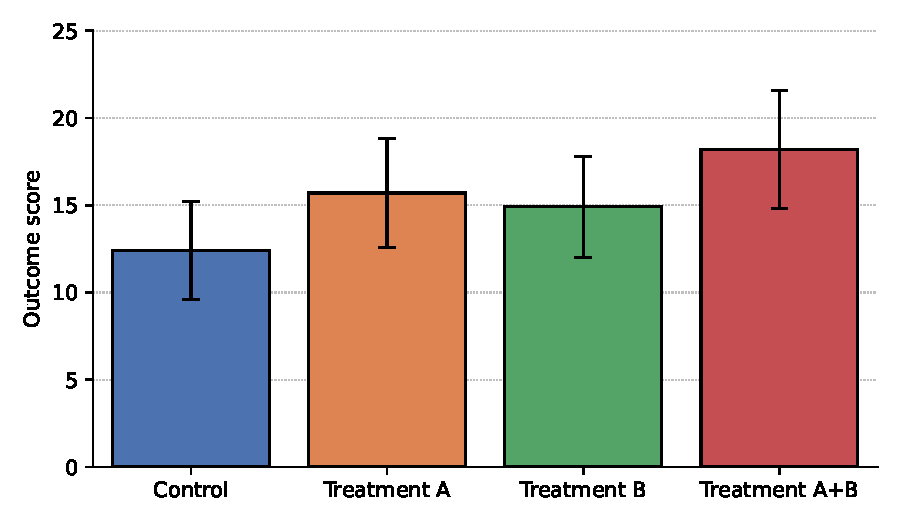
\includegraphics[width=0.7\textwidth,keepaspectratio]{assets/figures/fig_demo_colorbox.pdf}
  \caption{
    % figure title
    \textbf{Demo outcome score by study condition.}
    % figure summary
    Bar heights show the mean outcome score for each condition, with error
    bars indicating the standard deviation. Values match the synthetic
    dataset summarised in Table~\ref{tab:demo-descriptive} and exist to
    demonstrate how a figure asset is wrapped by a component file.
  }
  \label{fig:demo-colorbox}
  \end{minipage}
\end{figure}


% \subsection{Secondary analysis}

% [Secondary results and analysis]


Full texts of 13,434 articles published from 2005 to 2025 were collected from PubMed Central. 10,919 of them have supplementary files (3 files on average). After evaluation by LLM, 12,699 articles were found to be original MR researches and passed to STROBE-MR compliance assessment. Most of these (88.6\%) used two-sample designs. 10,641 studies were published after 2021 (when the STROBE-MR was first introduced) and 2,789(26.2\%) of them mentioned or cited STROBE-MR.
% \begin{figure}[H]
    \centering
    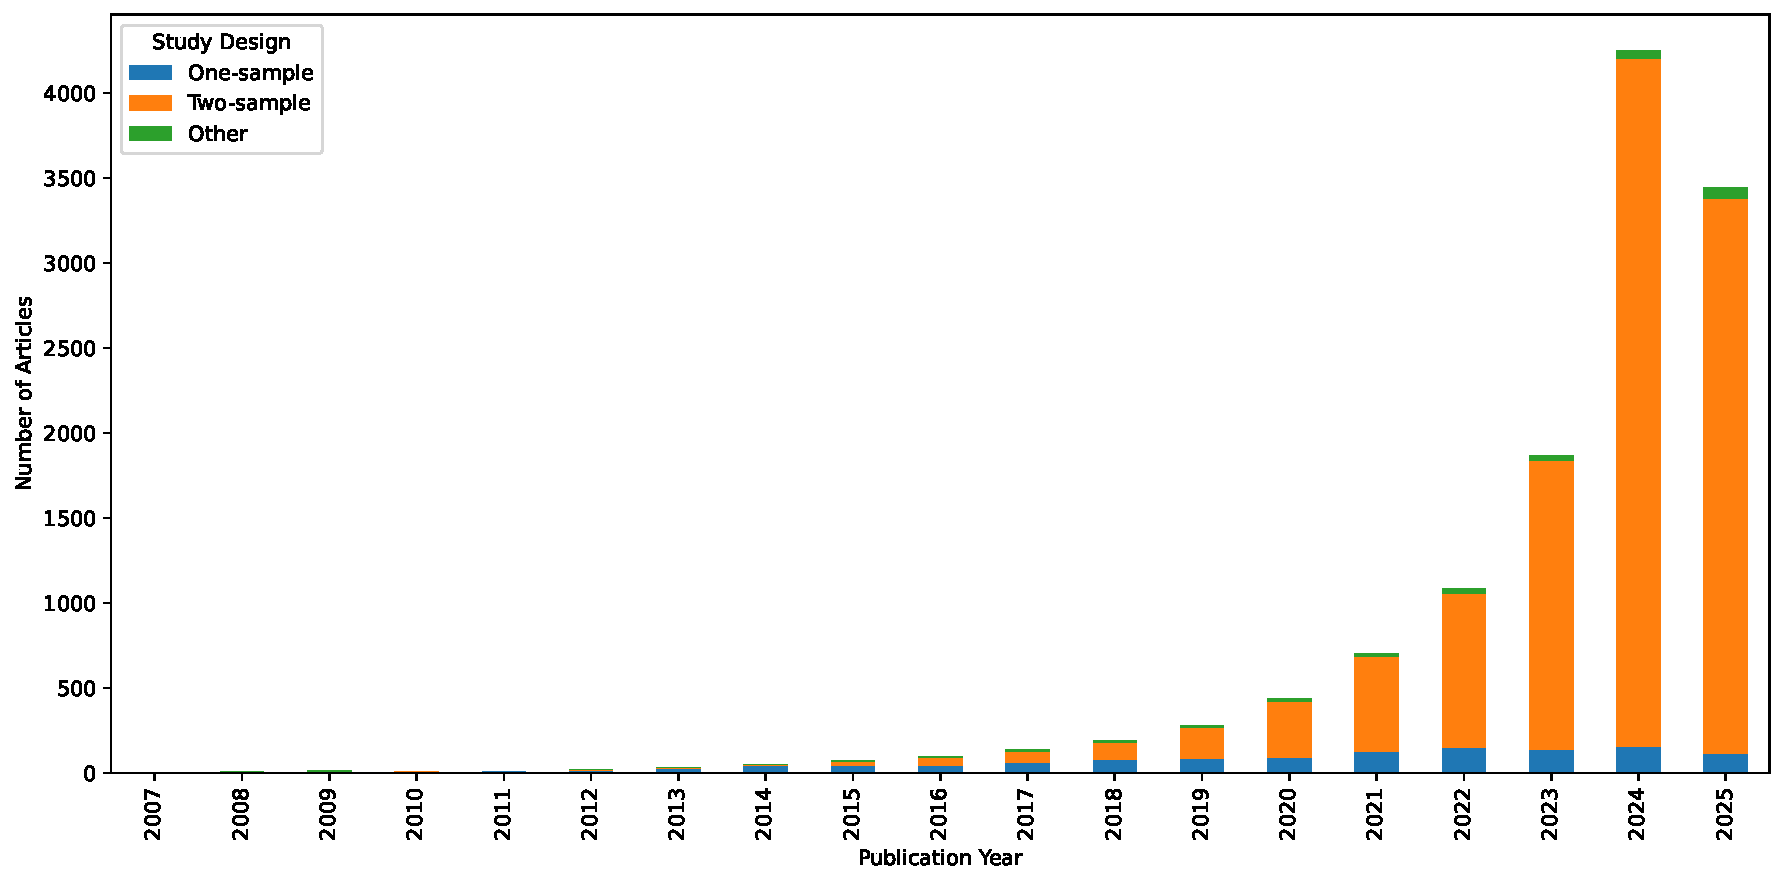
\includegraphics[width=0.8\linewidth]{assets/figures/general/study_design_by_year.pdf}
    \caption{Study design by publication year}
    \label{fig:study-design:year}
\end{figure}

\subsection{Model Evaluation}

46 studies were included in the final evaluation set (4 studies were excluded because MR was not the main purpose or they did not have human participants). 4 of them used one-sample designs while most of them (42) used two-sample designs. 36 studies were published after 2021, 10 of them (27.8\%) self-claimed to be compliant with STROBE-MR. However, no differences in the average number of items reported were found between studies with and without self-claimed compliance (both groups reported an average of 24 items). Table \ref{tab:eval:section} shows the distribution of grades for STROBE-MR components of the two reviewers. Reviewers have a maximal percentage of disagreement of 10.2\% and most of the disagreements occurred in the Methods and Results sections. 

Evaluation of the LLM's performance showed a high accuracy of 89.0\%. However, the accuracy decreased for items in the Methods and Results sections(see Table \ref{tab:model:accuracy}. This can be explained by the fact that these sections contain more technical details, the LLM has certain knowledge gaps, and the prompt did not provide enough information for the LLM to make correct decisions. For example, item 4c: "For each data source, describe measurement of genetic variants", this item requires articles to report the genotyping details, however, the LLM mixed up the measurement of genetic variants with the selection of genetic variants (p-value, LD clumping, etc.) and thus made wrong decisions. 

\begin{table}[h]
    \centering
    \caption{Annotation Summary by STROBE‑MR Section}
    \label{tab:eval:section}
    \begin{tabular}{llllllr}
    \toprule
    Section & Yes(JZ) (n, \%) & No(JZ) (n, \%) & Yes(YW) (n, \%) & No(YW) (n, \%) & Disagreement (n, \%) & Total (n) \\
    \midrule
    Title and Abstract & 46 (100.0\%) & 0 (0.0\%) & 46 (100.0\%) & 0 (0.0\%) & 0 (0.0\%) & 46 \\
    Introduction & 88 (95.7\%) & 4 (4.3\%) & 89 (96.7\%) & 3 (3.3\%) & 1 (1.1\%) & 92 \\
    Methods & 1067 (58.0\%) & 756 (41.1\%) & 1097 (59.6\%) & 719 (39.1\%) & 183 (9.9\%) & 1840 \\
    Results & 504 (57.7\%) & 337 (38.6\%) & 515 (58.9\%) & 338 (38.7\%) & 89 (10.2\%) & 874 \\
    Discussion & 406 (73.6\%) & 146 (26.4\%) & 424 (76.8\%) & 128 (23.2\%) & 20 (3.6\%) & 552 \\
    Other Information & 135 (48.9\%) & 139 (50.4\%) & 148 (53.6\%) & 121 (43.8\%) & 27 (9.8\%) & 276 \\
    \bottomrule
    \end{tabular}
\end{table}


\subsection{General Results}

On average, 22 of the 43 items of STROBE-MR were fully reported. The most frequently reported items were item 14: key results (99.3\%), item 1: title and abstract (98.5\%), item 16a: meaning of results (97.9\%), item 2: background (97.3\%), item 16c: clinical relevance (97.3\%), and item 8: sensitivity analysis (96.9\%). However, item 11c: translating to absolute risk (2.2\%), item 9b: registration of study (2.4\%), item 4b: paticipants (5.6\%), item 18: funding (6.3\%), and item 6c: details of MR estimator (8.7\%) were rarely reported among MR articles. Details can be found in Figure \ref{fig:meet:item}, results for each STROBE-MR component can be found in Table ~\ref{tab:report:component}. When comparing number of items reported in different year, we found it remained stable around 24 items. (Figure ~\ref{append:fig:meet:year}). However, the mean reporting number decreased from 24 items in 2021 to 21 items in 2025.
\begin{figure}[H]
    \centering
    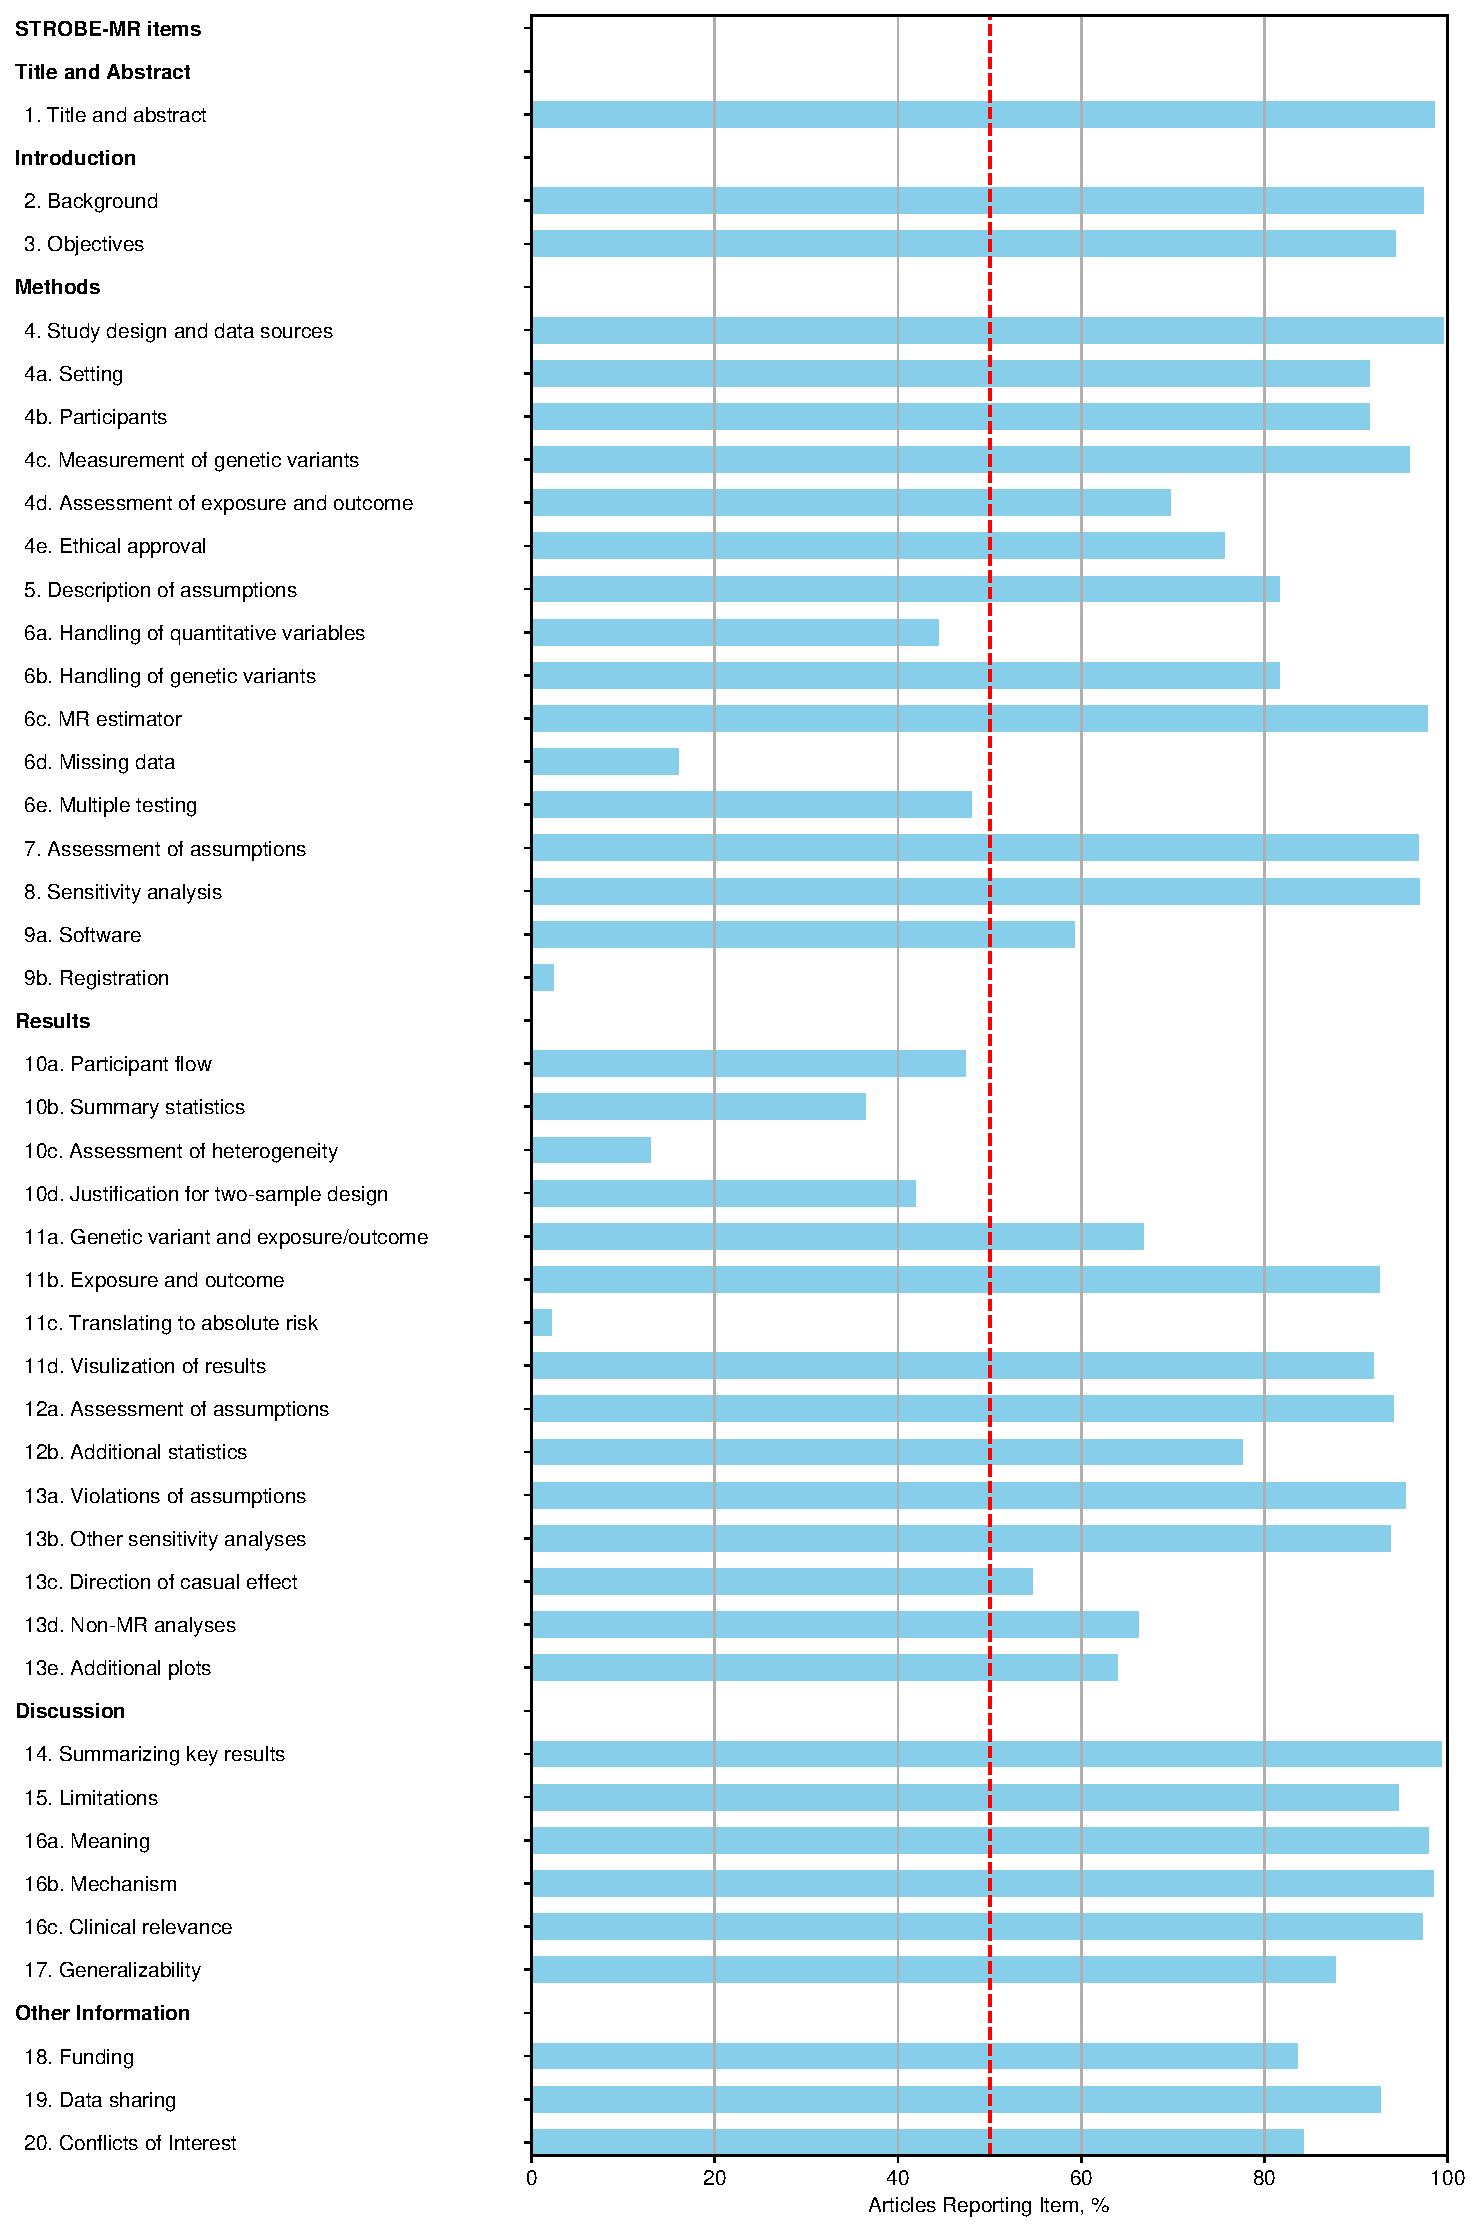
\includegraphics[width=0.8\textwidth,keepaspectratio]{assets/figures/subitem_all/meet_percentage_by_subitem.pdf}
    \caption{STROBE-MR reporting by item}
    \label{fig:meet:item}
\end{figure}
% \begin{figure}[H]
    \centering
    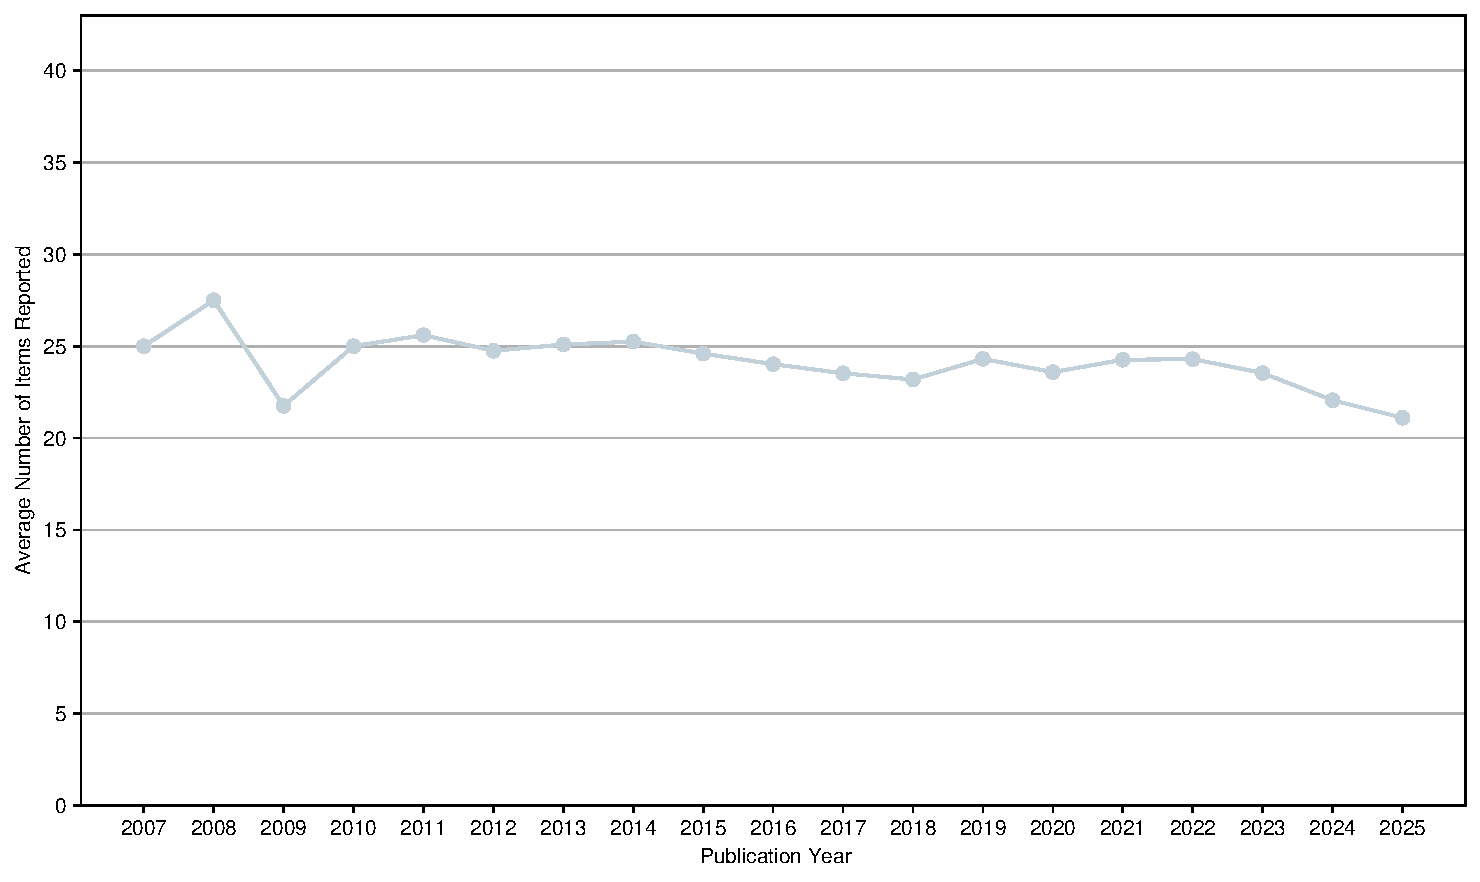
\includegraphics[width=0.8\linewidth]{assets/figures/subitem_all/avg_meet_num_by_year.pdf}
    \caption{STROBE-MR reporting by publication year}
    \label{fig:meet:year}
\end{figure}

\subsection{Reporting Trends in Different Sections}

The reporting rate of STROBE-MR items varied significantly in different sections. As we can see from Figure \ref{fig:meet:section}, items in Title/Abstract and Introduction sections were reported by most of the articles, with reporting rate of 98.5\% and 95.8\%, respectively. However, the reporting rates decreased significantly in other sections: followed by Results (51.3\%), Discussion (48.0\%) and Methods (32.8\%). Other Information section had the lowest reporting rate of 21.2\%. As we can see from Table ~\ref{tab:report:component}, there are only 24.5\% articles presented role of funders and 12.1\% of them shared statistical code. In Methods section, item 4b: paticipants and item 6c: details of MR estimator are rarely reported. 
In Discussion section, item 17: generalizability and item 16b: Mechanism are most likely missed by authors. 
Table ~\ref{tab:report:component} shows that gene-environment equivalence component of item 16b only has a reporting rate of 10.0\% and generalizability across other exposure periods and levels components of item 17 has reporting rates of 26.2\% and 20.0\%, respectively. 

Different temporal trends of reporting can also be observed in these sections (Figure \ref{fig:meet:section:year}). The reporting rates remained around 90\% in Title/Abstract and Introduction sections. Results section also had constant temporal trend but its reporting rate was only around 50\%. Methods, Discussion and Other Information sections all showed a decreasing trend, especially in recent years.
\begin{figure}[H]
    \centering
    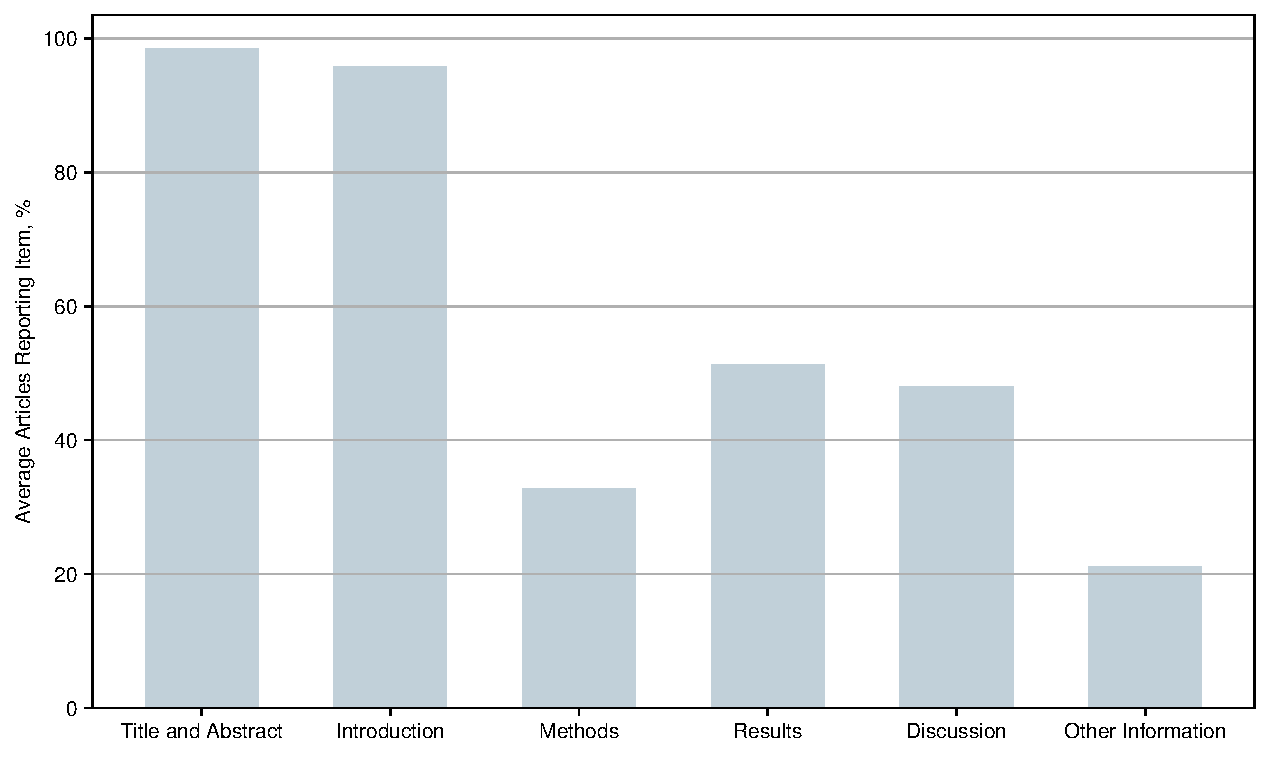
\includegraphics[width=0.8\linewidth]{assets/figures/subitem_all/meet_percentage_by_section.pdf}
    \caption{STROBE-MR reporting by section}
    \label{fig:meet:section}
\end{figure}
\begin{figure}[H]
    \centering
    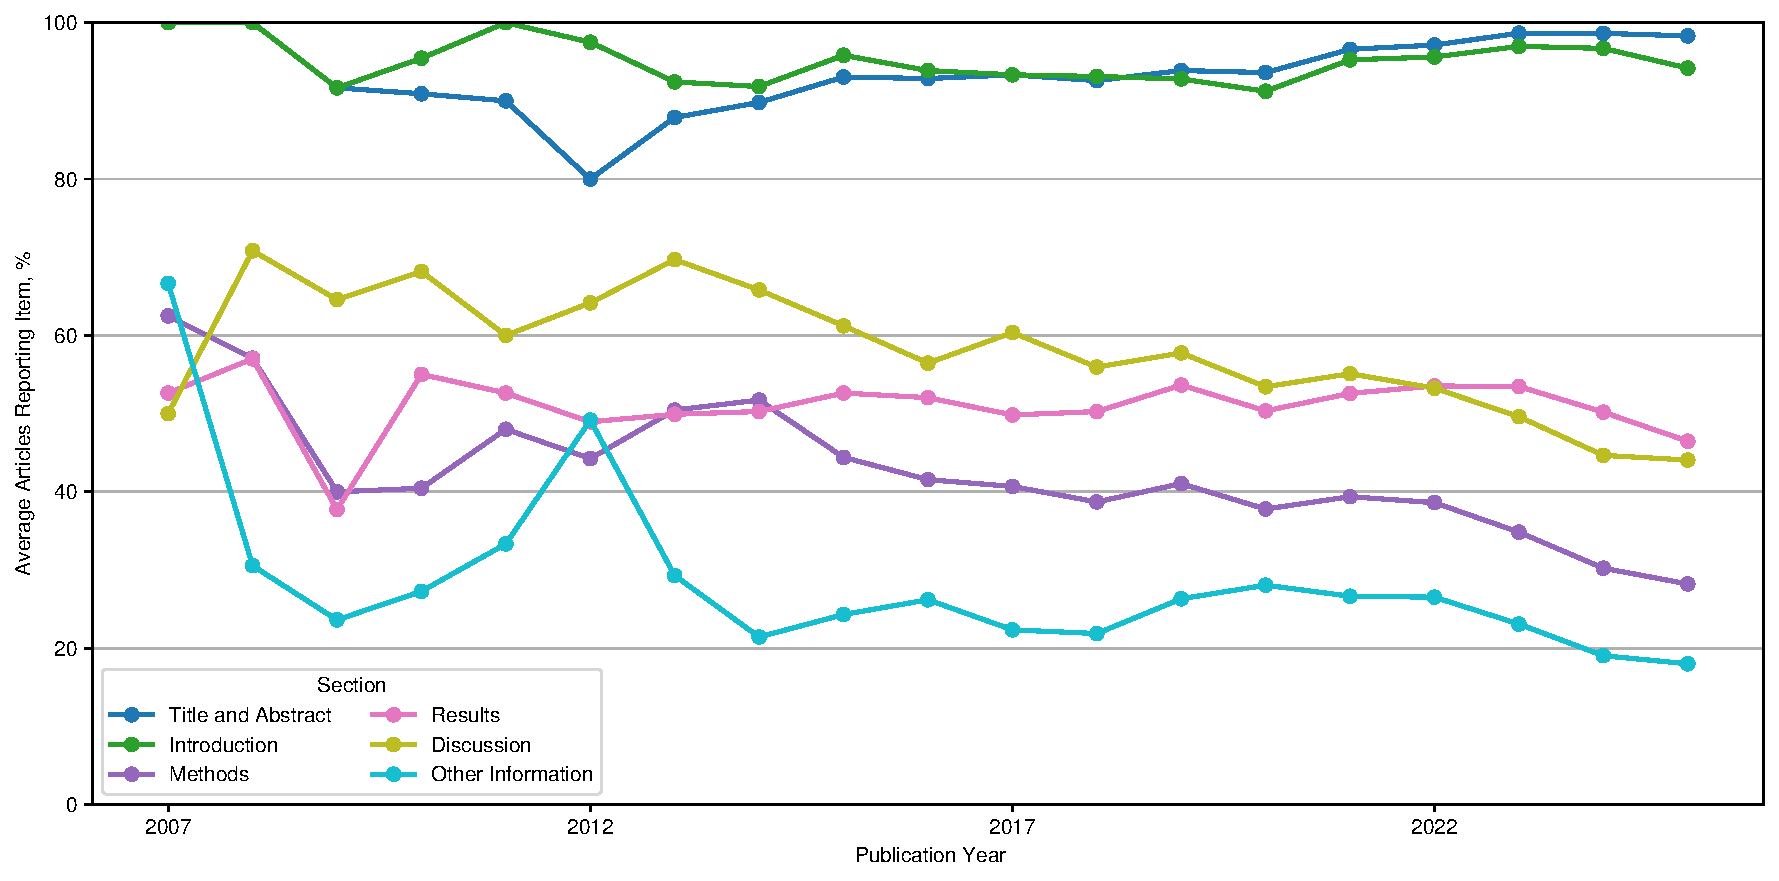
\includegraphics[width=0.8\linewidth]{assets/figures/subitem_all/meet_percentage_by_year_and_section.pdf}
    \caption{STROBE-MR reporting by year and section}
    \label{fig:meet:section:year}
\end{figure}

\subsection{Sensitivity Analysis}

Detailed results of the sensitivity analysis can be found in the Appendix. In general, the reporting rate of many items increased and the average number of items reported rose to 32. Figure \ref{append:fig:meet:year} shows there was a similar stable trend before 2021 and a decreasing trend after 2021. However, we observed significant changes in reporting rates of different items. The most frequently reported items were now item 4 (99.5\%), 14(99.3\%), 1(98.5\%), 16b(98.5\%) and 16a (98.0\%). The least reported items were item 11c(2.2\%), 9b(2.4\%), 10c(13.0\%), 6d(16.0\%), 10b(36.5\%). When comparing reporting rate in different sections, we observed a significant increase in the Methods (83.5\%), Discussion (94.8\%) and Other Information (86.7\%) sections. 
These are the least reported sections in the main analysis. We did not observe any temporal trends in most sections, because the reporting rates remained constant over the years. However, the reporting rate of Other Information rose from around 60\% to over 80\% in recent years. 


% Example cross-reference to supplementary materials
% Additional results are presented in Section~\ref{sec:supp-results} and Table~\ref{tab:supp-detailed-results} of the supplementary materials.
